\newpage
\section{Krisna Irawan}
\subsection{Purpose}
Our project is a proof of concept that intended to identify the feasibility of a new innovation technology for Rockwell Collins Head-Up Display (HUD) system. Rockwell Collins strive to improve their HUD installment process and accuracy. Currently, the instalment process of the HUD system is costly, time consuming and require specialized equipment and epoxy. This mechanical way of installing the HUD also created an in-flight accuracy problem caused by airframe droop. In this project we are evaluating the feasibility of having an additional MEMS IRU to reduce the instalment cost of the HUD and also eliminate the offset error caused by airframe droop. The end goal of this project is to create a demonstration system that utilize an additional MEMS IRU mounted onto the HUD to infer the alignment data from the aircrafts precisely mounted and aligned IRU. Our software system will produce an aligned data that compensate the alignment error correctly, and the alignment error should be within a range of one milliradian. We hope to find the alignment offset dynamically with this new methodology. By finding the alignment offset dynamically, Rockwell Collins can reduce the installment cost of their HUD and improve the accuracy of their HUD system during flight. 

\subsection{Current Stage}
I am in charge of the graphical user interface and the statistical analysis portion of the project. Currently, I am at the stage of connecting the graphical user interface that I created in Visual Studio to the offset algorithm part of the software created in Arduino by my teammates. At this stage, I make sure that the graphical user interface works smoothly by running a lot of user interface testing and configuration. I use a slider value in Visual Studio to make sure that the gauge works perfectly. I also put place holders for the alignment offset, original data, and offset data. I believe these place holders will reduce the time required for me when connecting the user interface and the offset algorithm in the future. The user interface runs smoothly with the visual studio environment. I am currently waiting for my teammates to make sure that their software portion in Arduino runs smoothly. I also have done research in connecting the Visual Studio graphical user interface with the Arduino environment. I am currently had a brief understanding with that process and probably will start to experiment with Arduino code next week. This week, I conducted a couple user study with my friends. Although the graphical user interface doesn’t look like a real HUD from Rockwell Collins, it still serves its purpose. See figure ~\ref{fig:hudsim} With a little explanation, my friends can grasp the concept and the meaning behind the HUD symbology in the user interface. I believe that at this stage the user interface is ready to go and I can move to the next implementation of the software. 

\begin{figure}
    \caption{The HUD Simulator}
    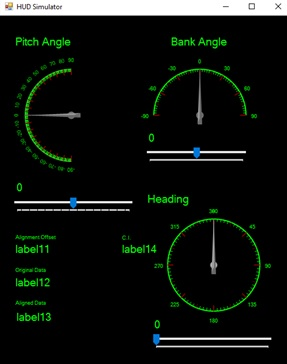
\includegraphics{img/hudsim}
    \label{fig:hudsim}
\end{figure}

\subsection{Remaining Work}
The next step for the user interface is to connect it to the Arduino part of the software. The hardware logistic problem at the beginning of the term has set our team behind the schedule for two weeks. This hinder our team ability to start working on the Arduino portion of the software. Currently, our team is still working on the hardware-software configuration part in Arduino. However, I believe with the current state the user interface, it will take a little time to connect it to the Arduino part of the software. I also would like to do more user study for the graphical user interface. There are significant changes in the user interface and I want to make sure that it still meets the standards of our client. I will start by confirming the user interface to our client this following week.

The next step on the implementation pipeline is the statistical analysis. I am in charged for the statistical analysis for both the pre-aligned data (the original data) and also the aligned data. I am still undecided on which IDE to write my code in. Currently, I am leaning towards to write my code in visual studio since I have been working with the Visual Studio IDE for the user interface. Last term I have done some research for statistical analysis method during the Tech Review. This term, I will start to do more research on the implementation side of the statistical analysis algorithm. The timeline for the statistical analysis portion of the software is tight. Hopefully I can finish the statistical analysis portion of the software on the next two weeks. 

\newpage
\subsection{Problems and Solutions}
There was a logistical problem at the beginning of the term. Our team were not able to get the hardware required to get started with this project. This problem was frustrating for our team since our project rely heavily with the hardware. Without the hardware it is not possible to get started with the bone and the core of this project. Our hardware is the most important part of the demonstration system. The hardware is where our team get the alignment data as the original data and data to be manipulated with the software.\\

To solve this problem, our team pro-actively contact the instructor and the TA to get the hardware. Our team sent a bunch of email reminding our instructor to get the hardware. Our team also tried to get in touch with the instructor in person. We came to the instructor office hour to talk about the hardware problem. We also talked about the hardware problem with the TA during meetings to see what our TA can do to help us. Our team also set up a meeting with the clients to let them know about the logistical problem that we were having. The meeting with the clients is important because it eliminates any misunderstanding that might happens between our team and our clients. This pro-active communication has allowed our team to get the necessary hardware faster and maintain our good relationship with the clients.\\

The logistical problem that happens at the beginning of the term has set us behind the schedule for 2 weeks. Our team got the necessary hardware at the beginning of week 3 and had to start with the implementation as soon as possible. To save time, our team decided to work in parallel. I was in charge of the graphical user interface portion of the software and my teammates were in charge in the hardware-software configuration. Because our team was working in parallel, everybody can start with their portion of the software. Hence, it saves our team a lot of implementation time. \\

At the beginning of the term, I thought that our clients will provide us with the HUD symbology that I can be imported to the graphical user interface. However, this wasn’t the case, our clients have a different method of generating the user interface on the HUD. Our clients used a software that will dynamically generate the HUD display. The Parameters come into the HUD software hosted on a computer via ethernet or Arinc- 429 inputs. Then software draws a distorted picture for the windshield and sent up to the HUD. This is significantly different than what I have in mind. There are no generic HUD symbology that I can directly import to the user interface. Thus, I have to create the HUD display from scratch. \\

Creating a HUD display is not an easy task. Rockwell Collins has put a lot of time and energy with their HUD display. Their current HUD display required a sophisticated software to generate it. Hence, creating a full HUD symbology will be out of scope of our project. I tried to be creative and use a gauge to act as the HUD symbology of the user interface. Although the gauge makes the user interface looks more like a car dashboard than an aircraft HUD, the user interface still serve it purpose in describing the data that we will get from our auto alignment system. 

\subsection{Interesting Code}
I use Visual Studio Toolkit to create the graphical user interface of the software. I wrote the code in C to make sure that it is compatible with Arduino. Because our team did not have the Arduino code ready, I decided to use the track bar as a method of debugging the graphical user interface. The track bar can be scrolled side by side to change the value of the gauge in the graphical user interface. To be able to use the gauge icon on the user interface, I imported a dll file called aGauge to my program. 

\begin{lstlisting}[language=c]
public Form1()
{
    InitializeComponent();
    label9.Text = "0";
    aGauge3.Value = 0;
    label10.Text = "0";
    aGauge2.Value = 0;
    label8.Text = "0";
    aGauge1.Value = 0;
}

private void Form1_Load(object sender, EventArgs e)
{
    trackBar1.Minimum = -90;
    trackBar1.Maximum = 90;
    trackBar1.TickStyle = TickStyle.BottomRight;
    trackBar1.TickFrequency = 1;
    trackBar3.Minimum = 0;
    trackBar3.Maximum = 360;
    trackBar3.TickStyle = TickStyle.BottomRight;
    trackBar3.TickFrequency = 1;
    trackBar2.Minimum = -90;
    trackBar2.Maximum = 90;
    trackBar2.TickStyle = TickStyle.BottomRight;
    trackBar2.TickFrequency = 1;
}

private void trackBar1_Scroll(object sender, EventArgs e)
{
    label9.Text = trackBar1.Value.ToString();
    aGauge3.Value = trackBar1.Value;
    aGauge3.Refresh();
}

private void trackBar2_Scroll(object sender, EventArgs e)
{
    label8.Text = trackBar2.Value.ToString();
    aGauge1.Value = trackBar2.Value;
    aGauge1.Refresh();
}

private void trackBar3_Scroll(object sender, EventArgs e)
{
    label10.Text = trackBar3.Value.ToString();
    aGauge2.Value = trackBar3.Value;
    aGauge2.Refresh();
}
\end{lstlisting}

\subsection{First User Study}
I conduct the user study with my friends. Although the graphical user interface doesn’t look like a real HUD from Rockwell Collins, it still serves its purpose. With a little explanation, my friends can grasp the concept and the meaning behind the HUD symbology in the user interface. I used gauge as the HUD symbology of the user interface. At first, it was slightly confusing since it is not a typical flight simulator HUD as figure ~\ref{fig:hudsimaction}. My friends told me that it looks more like a car dashboard. I will conduct the user study with our clients next week.  

\begin{figure}
 	\caption{The HUD Simulator in Action}
    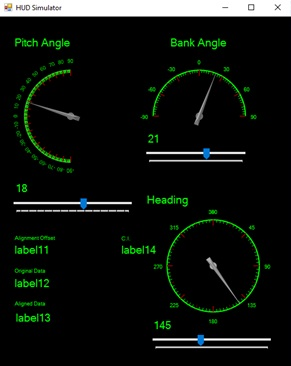
\includegraphics{img/hudsimaction}
    \label{fig:hudsimaction}
\end{figure}




